%%%%%%%%%%%%%%%%%%%%%%%%%%%%%%%%%%%%%%%%%
% Structured General Purpose Assignment
% LaTeX Template
%
% This template has been downloaded from:
% http://www.latextemplates.com
%
% Original author:
% Ted Pavlic (http://www.tedpavlic.com)
%
% Note:
% The \lipsum[#] commands throughout this template generate dummy text
% to fill the template out. These commands should all be removed when 
% writing assignment content.
%
%%%%%%%%%%%%%%%%%%%%%%%%%%%%%%%%%%%%%%%%%

%----------------------------------------------------------------------------------------
%	PACKAGES AND OTHER DOCUMENT CONFIGURATIONS
%----------------------------------------------------------------------------------------

\documentclass{article}

\usepackage{fancyhdr} % Required for custom headers
\usepackage{lastpage} % Required to determine the last page for the footer
\usepackage{extramarks} % Required for headers and footers
\usepackage{graphicx} % Required to insert images
\usepackage{lipsum} % Used for inserting dummy 'Lorem ipsum' text into the template
\usepackage{amsmath}
\usepackage{xcolor}

% Margins
\topmargin=-0.45in
\evensidemargin=0in
\oddsidemargin=0in
\textwidth=6.5in
\textheight=9.0in
\headsep=0.25in 

\linespread{1.1} % Line spacing

% Set up the header and footer
\pagestyle{fancy}
\lhead{\hmwkAuthorName} % Top left header
\chead{\hmwkClass\ (\hmwkClassInstructor\ \hmwkClassTime): \hmwkTitle} % Top center header
\rhead{\firstxmark} % Top right header
\lfoot{\lastxmark} % Bottom left footer
\cfoot{} % Bottom center footer
\rfoot{Page\ \thepage\ of\ \pageref{LastPage}} % Bottom right footer
\renewcommand\headrulewidth{0.4pt} % Size of the header rule
\renewcommand\footrulewidth{0.4pt} % Size of the footer rule

\setlength\parindent{0pt} % Removes all indentation from paragraphs

%----------------------------------------------------------------------------------------
%	DOCUMENT STRUCTURE COMMANDS
%	Skip this unless you know what you're doing
%----------------------------------------------------------------------------------------

% Header and footer for when a page split occurs within a problem environment
\newcommand{\enterProblemHeader}[1]{
    \nobreak\extramarks{#1}{#1 continued on next page\ldots}\nobreak
    \nobreak\extramarks{#1 (continued)}{#1 continued on next page\ldots}\nobreak
}

% Header and footer for when a page split occurs between problem environments
\newcommand{\exitProblemHeader}[1]{
    \nobreak\extramarks{#1 (continued)}{#1 continued on next page\ldots}\nobreak
    \nobreak\extramarks{#1}{}\nobreak
}

\setcounter{secnumdepth}{0} % Removes default section numbers
\newcounter{homeworkProblemCounter} % Creates a counter to keep track of the number of problems

\newcommand{\homeworkProblemName}{}
\newenvironment{homeworkProblem}[1][Problem \arabic{homeworkProblemCounter}]{ % Makes a new environment called homeworkProblem which takes 1 argument (custom name) but the default is "Problem #"
    \stepcounter{homeworkProblemCounter} % Increase counter for number of
% problems
    \renewcommand{\homeworkProblemName}{#1} % Assign \homeworkProblemName the
% name of the problem
    \section{\homeworkProblemName} % Make a section in the document with the
% custom problem count
    \enterProblemHeader{\homeworkProblemName} % Header and footer within the
% environment
}{
    \exitProblemHeader{\homeworkProblemName} % Header and footer after the
% environment
}

\newcommand{\problemAnswer}[1]{ % Defines the problem answer command with the content as the only argument
    \noindent\textbf{\emph{Answer: }}#1 % Just put a keyword Answer in
    % bold/italic at the beginning
}

\newcommand{\homeworkSectionName}{}
\newenvironment{homeworkSection}[1]{ % New environment for sections within homework problems, takes 1 argument - the name of the section
    \renewcommand{\homeworkSectionName}{#1} % Assign \homeworkSectionName to the
% name of the section from the environment argument
    \subsection{\homeworkSectionName} % Make a subsection with the custom name
% of the subsection
    \enterProblemHeader{\homeworkProblemName\ [\homeworkSectionName]} % Header
% and footer within the environment
}{
    \enterProblemHeader{\homeworkProblemName} % Header and footer after the
% environment
}

\newtheorem{theorem}{Theorem}[homeworkProblemCounter]
\newtheorem{lemma}[theorem]{Lemma}
\newtheorem{proposition}[theorem]{Proposition}
\newtheorem{corollary}[theorem]{Corollary}

\newenvironment{proof}[1][Proof]{
    \begin{trivlist}
        \item[\hskip \labelsep {\bfseries #1}]
    }{
        \end{trivlist}
}
\newenvironment{definition}[1][Definition]{
    \begin{trivlist}
        \item[\hskip \labelsep {\bfseries #1}]
    }{
        \end{trivlist}
}
\newenvironment{example}[1][Example]{
    \begin{trivlist}
        \item[\hskip \labelsep {\bfseries #1}]
    }{
        \end{trivlist}
    }
\newenvironment{remark}[1][Remark]{
    \begin{trivlist}
        \item[\hskip \labelsep {\bfseries #1}]
    }{
        \end{trivlist}
}

\newcommand{\qed}{
    \nobreak \ifvmode \relax \else
    \ifdim\lastskip<1.5em \hskip-\lastskip
    \hskip1.5em plus0em minus0.5em \fi \nobreak
    \vrule height0.75em width0.5em depth0.25em\fi
}
   
%----------------------------------------------------------------------------------------
%	NAME AND CLASS SECTION
%----------------------------------------------------------------------------------------

\newcommand{\hmwkTitle}{Assignment\ \#1} % Assignment title
\newcommand{\hmwkDueDate}{Tusday,\ January\ 13,\ 2015} % Due date
\newcommand{\hmwkClass}{ECS\ 222A} % Course/class
\newcommand{\hmwkClassTime}{TR 4:40pm-6:00pm} % Class/lecture time
\newcommand{\hmwkClassInstructor}{Daniel Gusfield} % Teacher/lecturer
\newcommand{\hmwkAuthorName}{Wenhao Wu} % Your name

%----------------------------------------------------------------------------------------
%	TITLE PAGE
%----------------------------------------------------------------------------------------

\title{
    \vspace{2in}
    \textmd{\textbf{\hmwkClass:\ \hmwkTitle}}\\
    \normalsize\vspace{0.1in}\small{Due\ on\ \hmwkDueDate}\\
    \vspace{0.1in}\large{\textit{\hmwkClassInstructor\ \hmwkClassTime}}
    \vspace{3in}
}

\author{\textbf{\hmwkAuthorName}}
\date{} % Insert date here if you want it to appear below your name

%----------------------------------------------------------------------------------------

\begin{document}

    \maketitle
    
    %----------------------------------------------------------------------------------------
    %	TABLE OF CONTENTS
    %----------------------------------------------------------------------------------------
    
    %\setcounter{tocdepth}{1} % Uncomment this line if you don't want subsections listed in the ToC
    
    \newpage
    \tableofcontents
    \newpage
    
    %----------------------------------------------------------------------------------------
    %	PROBLEM 1
    %----------------------------------------------------------------------------------------
    \begin{homeworkProblem}
        Given two strings $L$ and $S$ that have an equal number of occurrences
        of each specific character, we define $D(S_1, S_2)$ as the minimum number
        of transpositions of adjacent characters needed to convert $S_1$ into
        $S_2$. For example, $S_1 = CBADA$ can be converted into $S_2 = ABDCA$
        using exactly four transpositions. Notice that all the transpositions
        are done on $S_1$.
        
        \begin{homeworkSection}{\homeworkProblemName(a)}
            Assume that $S_1$ and $S_2$ each have exactly one occurrence of each
            character, for example $S_1 = ACBD$ and $S_2 = DCAB$. Develop an
            efficient algorithm to compute the number $D(S_1, S_2)$ given any
            input strings $S_1$ and $S_2$ that obey the stated assumption. Argue
            that your algorithm is correct (try to find a rigorous yet simple
            argument) and discuss how efficient it is in terms of the number of
            operations it does. (What are the primitive operations in your
            algorithm?)
            \vspace{10pt}
            
            \problemAnswer{
                \begin{lemma}
                    \label{lemma:1.1}
                    $D(S_1, S_2)$ equals to the Kendall tau distance between
                    $S_1$ and $S_2$, i.e.
                    \begin{align*}
                        D(S_1, S_2) & = K(S_1, S_2) \\
                         & = |\{(i,j)|i<j,(\tau_1[i]<\tau_1[j]
                        \mbox{ AND } \tau_2[i]>\tau_2[j]) \mbox{ OR }
                        (\tau_1[i]>\tau_1[j] \mbox{ AND }
                        \tau_2[i]<\tau_2[j])\}|
                    \end{align*}
                    where $\tau_1[i]$ and $\tau_2[i]$ denotes the index/ranking
                    of character $i$ in $S_1$ and $S_2$, respectively.
                \end{lemma}
                \begin{proof}
                    Firstly, each transpositions of adjacent characters in $S_1$
                    can at most reduce $K(S_1, S_2)$ by 1, and when $S_1$
                    is eventually converted to $S_2$ with transpositions $K(S_1,
                    S_2) = 0$. As a result, $K(S_1, S_2)$ is a lower
                    bound of $D(S_1, S_2)$.
                    
                    On the other hand, bubble sort uses exactly $K(S_1, S_2)$
                    adjacent transpositions to convert $S_1$ to $S_2$,
                    therefore $K(S_1, S_2)$ is achievable. Consequently, $D(S_1,
                    S_2) = K(S_1, S_2)$
                \end{proof}
                A classical algorithm to compute $K(S_1, S_2)$ is merge-sort,
                has $\mathcal{O}(n\log n)$ complexity. Define index sequence $Q$
                such that
                \[
                    Q[k] = \tau_1[S_2[k]],\,k=1,\ldots,n
                \]
                the constructing of which has $\mathcal{O}(n)$ complexity. Then
                we can simply count the number of inverted pairs in $Q$ using
                merge sort to compute $D(S_1, S_2)$.
            }
        \end{homeworkSection}
        
        \begin{homeworkSection}{\homeworkProblemName(b)}
            Develop an efficient algorithm to actually transform $S_1$ into
            $S_2$ using exactly $D(S_1, S_2)$ transpositions. Argue that your
            algorithm is correct and discuss how efficient it is in terms of the
            number of operations it does. The operations are the operations done
            by the algorithm, not the number of transpositions needed.
            \vspace{10pt}
            
            \problemAnswer{
                As stated in the proof to Lemma~\ref{lemma:1.1}, we can bubble
                sort $S_1$ based on the pairwise ranking defined by $Q$, which
                uses exactly $D(S_1, S_2)$ transpositions to convert $S_1$ to
                $S_2$, since each transposition reduces $D(S_1, S_2)$ exactly by
                1. It has $\mathcal{O}(n^2)$ complexity.
             }
        \end{homeworkSection}
        
        \begin{homeworkSection}{\homeworkProblemName(c)}
            Now explain how to handle the case of computing $D(S_1 , S_2)$ when
            those strings may have more than one occurrence of any character.
            Assume that both strings have the same number of occurrences of any
            particular character. Hint: One approach is to find a simple
            reduction of this problem to the previous one. Of course, give a
            proof of correctness and an analysis of the number of operations
            needed.
            \vspace{10pt}
            
            \problemAnswer{
                \begin{lemma}
                    \label{lemma:1.2}
                    The transpositions that achieve $D(S_1 , S_2)$ does not
                    change the order of multiple occurences of a same character.
                    In other words, assume there are $n_i$
                    occurences of character $i$ in $S_1$. After $S_1$ being
                    converted to $S_2$, each of this occurence appears in a new
                    position denoted as $c_1^{(i)},
                    c_2^{(i)},\ldots,c_{n_i}^{(i)}$, where the subscripts
                    denotes the order of their original appearance in $S_1$,
                    then a series of $D(S_1 , S_2)$-achieving transpositions
                    must satisfy
                    \[
                        c_1^{(i)}<c_2^{(i)}<\ldots<c_{n_i}^{(i)}
                    \]
                \end{lemma}
                \begin{proof}
                    If there exists $c_l^{(i)}>c_{l+1}^{(i)}$, then the $l$-th
                    and the $l+1$-th occurence of character $i$ must have been
                    transposed somewhere, which is totally unnecessary. This
                    is in contradict with the assumption of minimum number of
                    transposition.
                \end{proof}
                According to Lemma~\ref{lemma:1.2}, we can redefine the
                index/ranking for each occurence of each character. Denote
                $\tau_1[i, m]$ as the index of the $m$-th occurence of character
                $i$ in $S_1$, then the index sequence $Q$ is also redefined as
                \[
                    Q[k_2[i, m]] = \tau_1[i, m],\,k=1,\ldots,n
                \]
                where $k_2[i, m]$ is the index of the $m$-th occurence of
                character $i$ in $S_2$. Then counting the number of inverted
                pairs in $Q$ using merge sort results in $D(S_1, S_2)$.
                
                The algorithm to compute $D(S_1, S_2)$ and actually transform
                $S_1$ into $S_2$ is implemented in \textbf{\emph{hw\_1\_1.py}}.
            }
        \end{homeworkSection}
        
    \end{homeworkProblem}
    %\clearpage
    
    %----------------------------------------------------------------------------------------
    %	PROBLEM 2
    %----------------------------------------------------------------------------------------
    
    \begin{homeworkProblem}
        The following algorithmic problem arose in the field of Sociology. You
        are given two strings, for example $L = ABCCBCD$ and $S = AQCBAD$. For
        each character $X$ in the alphabet, define $M(X)$ as the minimum number
        of times $X$ appears in either $L$ or $S$. For example, $M(A) = 1$ and
        $M(Q) = 0$ in the example above.
        \\\\
        The problem requires us to remove characters from $L$ and $S$ so that
        for each character $X$, the number of remaining occurrence of $X$ in
        each of $L$ and $S$ is exactly $M(X)$. So far there is no real problem
        since we know exactly how many of each character must be removed from
        each string.
        \\\\
        However, for some character(s) $X$ there may be choices for which
        specific occurrences of $X$ should be removed. Hence there are choices
        for what the resulting strings (call them $S_1$ and $S_2$) will be.
        \\\\
        Now comes the problem: Among all possible ways to choose the required
        removals, we want to create resulting strings $S_1$ and $S_2$ to
        minimize $D(S_1, S_2)$. We call this the \emph{MinDistRem problem}. For
        example, with $L$ and $S$ above, we can create $S_1 = ABCD$ and $S_2 =
        CBAD$ with $D(S_1, S_2) = 3$, or we could create $S_1 = S_2 = ACBD$ with
        $D(S_1, S_2) = 0$, and so we choose the latter as the solution to the
        \emph{MinDistRem} problem.

        \begin{homeworkSection}{\homeworkProblemName(a)}
            Solve the MinDistRem problem for $L = ACDQDCGFDERAE$ and $S =
            EECDACWERGARF$.
            \vspace{10pt}
            
            \problemAnswer{
                Denote $H_L[X]$ and $H_S[X]$ as the number of occurences of
                character $X$ in string $L$ and $S$, respectively. We have
                \begin{table}[!h]
                    \renewcommand{\arraystretch}{1.3}
                    %\caption{}
                    %\label{}
                    \centering
                    \begin{tabular}{c|ccc}
                        \hline
                        $X$ & $H_L[X]$ & $H_S[X]$ & M[X] \\
                        \hline
                        A & 2 & 2 & 2 \\
                        C & 2 & 2 & 2 \\
                        D & 3 & 1 & 1 \\
                        E & 2 & 3 & 2 \\
                        F & 1 & 1 & 1 \\
                        G & 1 & 1 & 1 \\
                        Q & 1 & 0 & 0 \\
                        R & 1 & 2 & 1 \\
                        W & 0 & 1 & 0 \\
                        \hline
                    \end{tabular}
                \end{table}
                We first note that ``Q'' must be removed from $L$ and ``W'' must
                be removed from $S$, while ``A'', ``C'', ``F'' and ``G'' should
                not be removed. 2 ``D'' must be removed from ``L'', 1 ``E'' must
                be removed from $S$ and 1 ``R'' must be removed from $S$. We
                remove the characters that are surely to be removed and
                highlight the characters that could be removed as 
                \begin{align*}
                    L & = AC\textcolor{blue}{DD}CGF\textcolor{blue}{D}ERAE \\
                    S & =
                    \textcolor{blue}{EE}CDAC\textcolor{blue}{ER}GA\textcolor{blue}{R}F
                \end{align*}
                There are a 3 ways of removing 2 ``D''s from $L$ and $2\times 2$
                ways to remove a ``E'' and ``R'' from S. We list the
                $D(S_1,S_2)$ for each possible pair of $S_1$ and $S_2$ in
                Table~\ref{table:DS1S2}
                \begin{table}[!h]
                    \renewcommand{\arraystretch}{1.3}
                    \caption{All possible $D(S_1,S_2)$ for exhaustive search.}
                    \label{table:DS1S2}
                    \centering
                    \begin{tabular}{c|cc}
                        \hline
                        $S_2$ & $S_1=ACCGFDERAE$ & $S_1=ACDCGFERAE$ \\
                        \hline
                        $ECDACEGARF$ & 18 & 15 \\
                        $ECDACERGAF$ & 18 & 15 \\
                        $EECDACGARF$ & 22 & 19 \\
                        $EECDACRGAF$ & 22 & 19 \\
                        \hline
                    \end{tabular}
                \end{table}
                
                Using an exhaustive search, we have $S_1 = ACCGFDERAE$ and $S_2
                = ECDACERGAF$ or $S2 = ECDACEGARF$.
            }
        \end{homeworkSection}
    
        \begin{homeworkSection}{\homeworkProblemName(b)}
            We would like to find an efficient algorithm for the MinDistRem
            problem. The following algorithm was proposed:
            \begin{enumerate}
                \item Let $L$ be the longer string and $S$ the shorter string.
                If the two strings are the same length, choose $L$ and $S$
                arbitrarily.
                \item For string $L$ make a list (called LIST, duh!) of the
                characters (but not their positions) that will be removed. For
                each such character $X$ include on LIST a number of copies of
                $X$ equal to the number of occurrences of $X$ that must be
                removed.
                \item Set pointer $p$ to 1 and pointers $q$ and $q'$ to 0.
                \item Let $X$ be the character in position $p$ of $S$.
                \item Scan $L$ for the first occurrence (if any) of character
                $X$ from position $p$ forward in $L$. If such an $X$ is found,
                set $q'$ to the position of that found $X$.
                \item If such an $X$ was found in $L$, scan the characters from
                $q + 1$ to $q' - 1$ (inclusive) for any characters on the LIST.
                As each such character is found (if any are) remove it from $L$
                and remove one copy of it from the LIST.
                \item Set $q$ to $q'$.
                \item Increment $p$ by one.
                \item Repeat steps 5 through 8 until $p$ is at the end of $S$ or
                until LIST is empty.
                \item If LIST is not empty, scan $L$ from its right end to find
                occurrences of characters on LIST. As each such character is
                found (if any are), remove it from $L$ and remove one copy of it
                from LIST.
                \item If sequence $L$ is now shorter than sequence $S$, exchange
                the labels $L$ and $S$, and repeat steps 2 to 10 on these two
                current strings $L$ and $S$. Else terminate.
                \item At termination, one the remaining string $L$ is called
                $S_1$ and the remaining string $S$ is called $S_2$.
            \end{enumerate}
            \problemAnswer{
                This algorithm is implemented in \textbf{\emph{hw\_1\_2.py}}.
            
            }
        \end{homeworkSection}
    
        \begin{homeworkSection}{\homeworkProblemName(c)}
            Execute the above algorithm on $L = ABCCBCD$ and $S = ACBAD$
            and then on $L = ACDQDCGFDERAE$ and $S = EECDACWERGARF$.
            \vspace{10pt}
            
            \problemAnswer{
                On $L = ABCCBCD$ and $S = ACBAD$ the glorithm results in $S_1 =
                S_2 = ACBD$.  On $L = ACDQDCGFDERAE$ and $S = EECDACWERGARF$
                the algorithm results in $S_1 = ECDACEGARF$ and $S_2 =
                ACCGFDERAE$.
            }
        \end{homeworkSection}
    
        \begin{homeworkSection}{\homeworkProblemName(d)}
            Argue that the algorithm always terminates within two executions of
            steps 2 to 10.
            \vspace{10pt}
            
            \problemAnswer{
                Steps 2 to 10 removes characters from $L$. Since step 10 ensures
                all characters in LIST are removed, and from the definition
                of LIST in step 2, the occurence of each character $X$ in $L$ is
                exactly $M[X]$ now. 
                \\\\
                Since $S$ has not been altered yet, if $S$ is in the same length
                as $L$, then the occurence of each character $X$ in $S$ is
                exactly $M[X]$ now and there is nothing to remove from it, the
                algotithm terminates in one pass of step 2 to 10. Otherwise the
                by swapping $L$ and $S$ the second pass will ensure so.
                Consequently, the algorithm always terminates within two
                executions of steps 2 to 10.
             }
        \end{homeworkSection}
        
        \begin{homeworkSection}{\homeworkProblemName(e)}
            Is it true that the algorithm always solves the MinDistRem problem?
            Justify.
            \vspace{10pt}
            
            \problemAnswer{
             }
        \end{homeworkSection}
    \end{homeworkProblem}
    
    %----------------------------------------------------------------------------------------
    %	PROBLEM 3
    %----------------------------------------------------------------------------------------
    
    \begin{homeworkProblem}    
        If you think the above algorithm does not solve the MinDistRem problem,
        can you propose an efficient algorithm that does always solve it? (this
        may be a very hard problem)
        \vspace{10pt}
            
        \problemAnswer{
        }
    \end{homeworkProblem}
    
    %----------------------------------------------------------------------------------------
    %	PROBLEM 4
    %----------------------------------------------------------------------------------------
    
    \begin{homeworkProblem}
        A ``prototein'' is a binary string that we embed on a two-dimensional
        grid. A legal embedding must satisfy the following rules:
        \begin{enumerate}
            \item Each character in the string gets placed on one point of the
            grid.
            \item Each point of the grid gets at most one character of the
            string placed on it.
            \item Two adjacnet characters in the string must be placed on two
            points that are neighbors on the grid in either the horizontal or
            vertical direction, but not both. That is, two points across a
            diagonal are not neighbors. (Note that an interior point on the grid
            has four neighbor on the grid, and that an outside point has three
            neighbors, and that a corner point has only two neighbors).
        \end{enumerate}
        Rules 1,2,3 mean that we are embedding the string onto the grid as a
        self-avoiding walk, without deforming the string. See the figure below.
        \begin{figure}[!h]
            \centering
            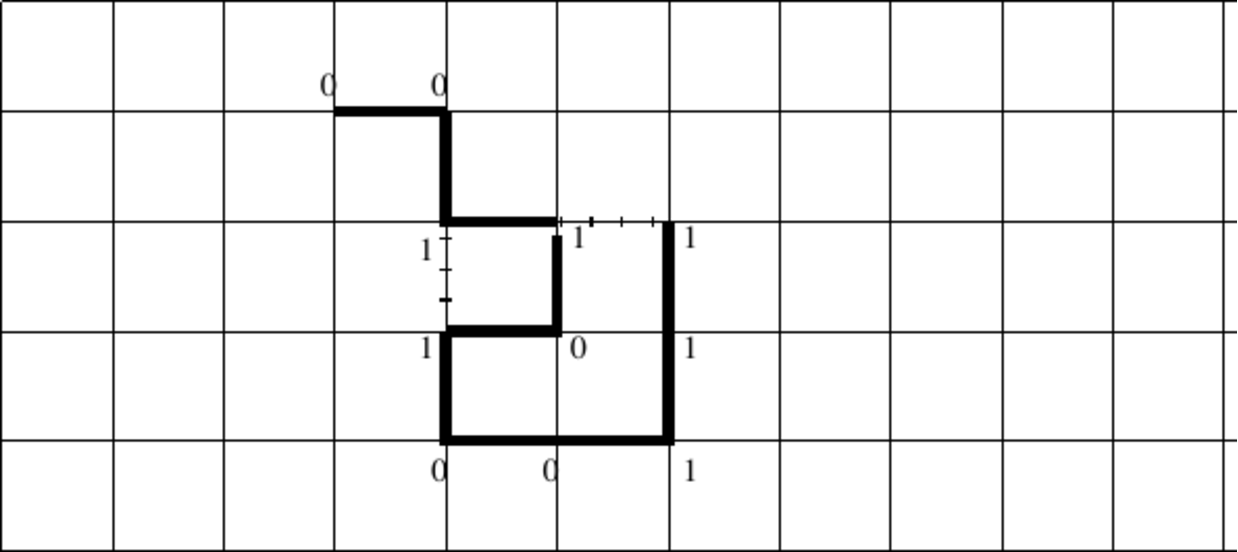
\includegraphics[width=0.75\columnwidth]{figs/fig_1.pdf}
            \caption{One possible embedding of the string 00110100111. The
            hatched lines show the contacts, two in this embedding. Can you find
            an embedding with more contacts?}
            \label{fig:fig_1}
        \end{figure}
        A contact is formed for every pair of 1's that are not adjacent in the
        string, but are placed on neighboring points in the grid. Such a pair of
        1's is called a ``contact'' in the embedding.
        \\\\
        Given an input string, the general problem is to find an embedding of
        the string on the grid so as to maximize the number of contacts.
        \\\\
        Your Problems:
        
        \begin{homeworkSection}{\homeworkProblemName(a)}
            Prove (that is give a clear explanation for) the following claim:
            For any string, and any legal embedding of the string, the
            characters in positions $i$ and $j$ in the string can form a contact
            only if $|i − j|$ is odd. Try playing with some examples first to
            convince yourself that this is true, and then try to find a concise
            way to prove it.
            \vspace{10pt}
            
            \problemAnswer{
            }
        \end{homeworkSection}
        
        \begin{homeworkSection}{\homeworkProblemName(b)}
            For any given string $S$, let $E(S)$ be the number of 1's in even
            positions in the string, and let $O(S)$ be the number of 1's in odd
            positions in the string. Let $C(S)$ be the minimum of $E(S)$ and
            $O(S)$. Prove that the number of contacts, in any legal embedding of
            $S$, cannot exceed $2(C(S) + 1)$.
            \vspace{10pt}
            
            \problemAnswer{
            }
        \end{homeworkSection}
        
        \begin{homeworkSection}{\homeworkProblemName(c)}
            If we can invent the string $S$, as well as decide on how to embed
            it, we could get alot of contacts, but that is cheating. Still if we
            can invent a string $S$, and embed it, so that the ratio of the
            number of contacts to the number of 1's in the string is high, that
            would be a good challenge. Find a string $S$, and an embedding of
            it, that has a ratio of contacts to 1's of $7/6$. Hint: you will
            need a string of length more than 25 (I think). So you will have to
            discover an idea, rather than just playing around.
            \vspace{10pt}
            
            \problemAnswer{
            }
        \end{homeworkSection}
        
        \begin{homeworkSection}{\homeworkProblemName(d)}
            Prove that, over all possible strings and embeddings of those
            strings, the highest possible ratio of contacts to 1's is $7/6$.
            Hint: the handshake lemma from graph theory (remember graphs from
            cs100 or cs20?) is helpful here. The rest is just case analysis.
            \vspace{10pt}
            
            \problemAnswer{
            }
        \end{homeworkSection}
    \end{homeworkProblem}
    
    %----------------------------------------------------------------------------------------

\end{document}